\documentclass{article}

\usepackage{subfig}
\usepackage{tikz}

\usepackage{amsmath}
\usepackage{listings}
\usepackage{algorithm}
\usepackage[noend]{algpseudocode} %for pseudo code, include algorithmicsx automatically

% for better Haskell code outlook
\lstdefinelanguage{Haskell}{
  basicstyle=\small\ttfamily,
  flexiblecolumns=false,
  basewidth={0.5em,0.45em},
  literate={+}{{$+$}}1 {/}{{$/$}}1 {*}{{$*$}}1 {=}{{$=$}}1
           {>}{{$>$}}1 {<}{{$<$}}1 {\\}{{$\lambda$}}1
           {\\\\}{{\char`\\\char`\\}}1
           {->}{{$\rightarrow$}}2 {>=}{{$\geq$}}2 {<-}{{$\leftarrow$}}2
           {<=}{{$\leq$}}2 {=>}{{$\Rightarrow$}}2
           {\ .}{{$\circ$}}2 {\ .\ }{{$\circ$}}2
           {>>}{{>>}}2 {>>=}{{>>=}}2
           {|}{{$\mid$}}1
}[keywords,comments,strings]

\lstloadlanguages{C, Haskell, Python}

\lstset{
  showstringspaces = false
}

\begin{document}

\title{Circular linked-list, A cycle detection problem}
\author{Larry LIU Xinyu}
\maketitle

\section{The problem}

In imperative settings, a linked-list may be corrupted, that it is circular. In such a list, some node
points back to previous one. Figure \ref{fig:circular-list} shows such situation.
The normal iteration ends up infinite looping.
  \begin{enumerate}
    \item Write a program to detect if a linked-list is circular;
    \item Write a program to find the node where the loop starts (the node being pointed by two precedents).
  \end{enumerate}

\begin{figure}[htbp]
\centering
\begin{tikzpicture}[scale=3]
  % trace
  \draw[dashed, very thin] (-2cm, 1cm) -- (0, 1cm);
  \draw[dashed, very thin] (0,0) circle [radius=1cm];

  % leading nodes
  \foreach \x in {-2, -1.7, ..., -1.4} {
    \draw[thick] (\x cm, 1cm) +(-0.1, -0.1) rectangle ++(0.1, 0.1);
    \draw[thick, ->] (\x cm, 1cm) -- +(0.2, 0);
  }

  % cricular starting points
  \draw[thick, ->] (-0.3cm, 1cm) -- (-0.1cm, 1cm);

  % circular nodes
  \foreach \deg/\rot in {90/0, 60/-30, 30/-60, 0/-90, 180/90, 150/60, 120/30} {
    \draw[thick] (\deg : 1cm) +(-0.1, -0.1) rectangle ++(0.1, 0.1);
    \draw[thick, ->] (\deg : 1cm) -- +(\rot : 0.2);
  }
\end{tikzpicture}
\caption{A circular linked-list}
\label{fig:circular-list}
\end{figure}

The brute-force solution utilizes extra spaces to record the nodes being visited so-far.
When visits a node, if it has been visited, then the linked-list is circular, and this
node is the staring point of the loop. When arrives at the tail, the linked-list isn't
circular. This method isn't good enough. The space required is $O(n)$, where $n$ is the
number of nodes in the list. Depends on what data-structure is used to store
the visited nodes, the performance varies from $O(n \lg n)$ (using tree-set) to quadratic $O(n^2)$
(using list for example).

\section{Floyd's algorithm}

Consider a clock. The hand of hours rotates slower than the hand of minutes. Starts
from 12:00, they meets 12 times before the next 12:00. For this problem,
we can mimic the clock hands by two pointers. They iterate in different speed.
If there is a loop in a linked-list, the slower pointer must be caught by the faster
one at some time.

But we must be careful when extend from the continuous case (the clock example) to
the discrete case. Because the faster one may skip past the slower one \cite{Stepanov09}, \cite{TAOCP2}.
For some circle contains $n$ nodes, the
slower pointer iterates $k$ nodes a step, the faster pointer iterates $m$ nodes a step.
Where $n$, $m$, $k$ are all natural numbers. What if $am \not\equiv bk \pmod n$ for
any integer $a, b$? Can you deduce the solution constraint for this linear congruence equation?

We can set the slower speed as $v_s = 1$ node per step,
and the faster speed as $v_f = 2$ nodes per step. Starts from the head of the linked-list, if they
meet at some time, the linked-list is circular. Otherwise, if the faster pointer
arrives at or goes beyond the tail, the linked-list isn't circular.

\begin{algorithmic}[1]
\Function{Circular?}{$L$}
  \State $p \gets q \gets L$
  \While{$p \neq $ NIL $\land q \neq$ NIL}
    \State $p \gets$ \Call{Next}{$p$}
    \State $q \gets$ \Call{Next}{$q$}
    \If{$q=$ NIL}
      \State break
    \EndIf
    \State $q \gets$ \Call{Next}{$q$}
    \If{$p = q$}
      \State \Return True
    \EndIf
  \EndWhile
  \State \Return False
\EndFunction
\end{algorithmic}

The following ANSI C example program implements this method.

\lstset{language=C}
\begin{lstlisting}
int is_circular(struct Node* h) {
    struct Node *a, *b;
    a = b = h;
    while (a && b) {
        a = a->next;
        b = b->next;
        if (!b)
            break;
        b = b->next;
        if (a == b) return 1;
    }
    return 0;
}
\end{lstlisting}

Suppose there are two runners. One runs two times faster than the other, If they start
running at some point in a circular stadium, when they meet again? The answer is the
same starting point. The faster runner runs 2 circles and the the slower runner runs
one circle when they meet again.

But for this problem, the situation is a bit different. The two 'runners' don't
start racing both at point $A$ as shown in figure \ref{fig:circular-catching}.
When the slower pointer arrives
at $A$, the faster one is at point $B$. Because the speed $v_f = 2v_s$, we have
$|OA| = |AB|$ if the circumference is longer than $|OA|$.
Denote the node where the circle start as the $k$-th one, the
faster pointer starts at the $2k$-th node when this 'racing' begins. Because it's
a circle, the faster pointer runs after the slower one with distance of $n-k$ nodes.

Here we only consider the case that $k < n$, we'll explain the $k \geq n$ case next.

The time it takes when the two pointers meet again can be gotten by dividing the distance by
the difference of their speed:

\begin{equation}
\begin{array}{rlr}
T & = \displaystyle \frac{n-k}{v_f - v_s} & \\
  & = \displaystyle \frac{n-k}{v_s} & (\textrm{since } v_f = 2v_s)
\end{array}
\end{equation}

So when the two pointers meet, the distance that the slower pointer runs is $Tv_s = n - k$.

It means that the meet point is the $k$-th node before $A$ around the circle.
The only unknown value
is $k$ at this stage. Observe that point $A$ is the $k$-th node from $O$ as well.
We can solve this problem with the following approach.

\begin{enumerate}
\item Use two pointers $p$, and $q$. Start from the head of the linked-list. $p$ iterates
a node per step, while $q$ iterates two nodes per step;
\item If there is a loop, $p$ and $q$ will meet. Reset $q$ to the head of the linked-list;
\item Advance $p$ and $q$ one node per step at the same time till they meet at $A$. Both
pointer point to the node where the loop starts.
\end{enumerate}

\begin{figure}[htbp]
\centering
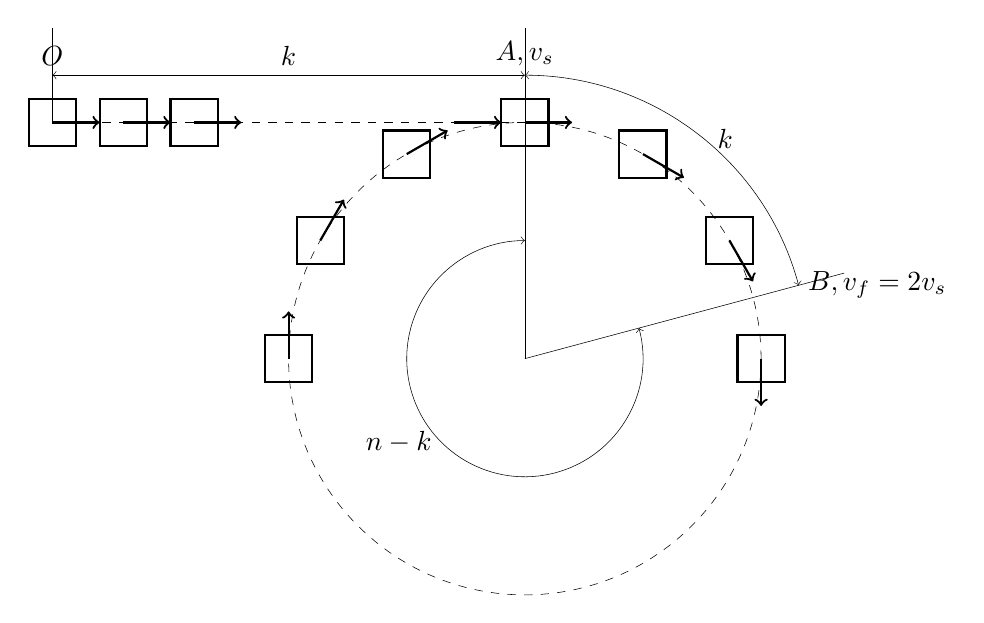
\begin{tikzpicture}[scale=3]
  % trace
  \draw[dashed, very thin] (-2cm, 1cm) -- (0, 1cm);
  \draw[dashed, very thin] (0,0) circle [radius=1cm];

  % label line
  \draw[very thin] (0, 0) -- (0, 1.4cm);
  \draw[very thin] (0, 0) -- (15:1.4cm);
  \draw[very thin] (-2cm, 1cm) -- +(0, 0.4cm);

  % label and arrows
  \draw[very thin, <->] (-2cm, 1.2cm) node[above]{$O$} -- (-1cm, 1.2cm) node[above]{$k$} -- (0, 1.2cm) node[above]{$A, v_s$};
  \draw[very thin, <->] (0, 1.2cm) arc [start angle = 90, end angle = 15, radius=1.2cm] node[right]{$B, v_f = 2v_s$};
  \draw (45:1.2cm) node[above]{$k$};
  \draw[very thin, <->] (15:0.5cm) arc [start angle = 15, end angle = -270, radius=0.5cm];
  \draw (-135:0.5cm) node[left]{$n-k$};

  % leading nodes
  \foreach \x in {-2, -1.7, ..., -1.4} {
    \draw[thick] (\x cm, 1cm) +(-0.1, -0.1) rectangle ++(0.1, 0.1);
    \draw[thick, ->] (\x cm, 1cm) -- +(0.2, 0);
  }

  % cricular starting points
  \draw[thick, ->] (-0.3cm, 1cm) -- (-0.1cm, 1cm);

  % circular nodes
  \foreach \deg/\rot in {90/0, 60/-30, 30/-60, 0/-90, 180/90, 150/60, 120/30} {
    \draw[thick] (\deg : 1cm) +(-0.1, -0.1) rectangle ++(0.1, 0.1);
    \draw[thick, ->] (\deg : 1cm) -- +(\rot : 0.2);
  }
\end{tikzpicture}
\caption{Two pointers solution.}
\label{fig:circular-catching}
\end{figure}

Let's consider the case that $k \geq n$. When the slower pointer arrives at $A$, The faster
one points to $B$ which is $k \bmod n$ nodes ahead. The faster one will catch
the slower one by eliminating their distance of $n - (k \bmod n)$ nodes.

\begin{equation}
\begin{array}{rl}
T & = \displaystyle \frac{n - (k \bmod n)}{v_f - v_s}\\
  & = \displaystyle \frac{n - (k \bmod n)}{v_s}
\end{array}
\end{equation}

When they meet again, the slower pointer has passed $v_sT = n - (k \bmod n)$ nodes.
The meet point is $k \bmod n$ nodes before $A$. We have the same result, that if
we reset the faster pointer to the head of the linked-list, and make the two pointers
advance one node per step, they will meet at $A$.

The following algorithm locates the node where the loop starts.

\begin{algorithmic}[1]
\Function{Find-Loop}{$L$}
  \State $p \gets q \gets L$
  \While{$p \neq $ NIL $\land q \neq$ NIL}
    \State $p \gets$ \Call{Next}{$p$}
    \State $q \gets$ \Call{Next}{$q$}
    \If{$q=$ NIL}
      \State break
    \EndIf
    \State $q \gets$ \Call{Next}{$q$}
    \If{$p = q$}
      \State $q \gets L$
      \While{$p \neq q$}
        \State $p \gets$ \Call{Next}{$p$}
        \State $q \gets$ \Call{Next}{$q$}
      \EndWhile
      \State \Return $p$ \Comment{Or return $q$}
    \EndIf
  \EndWhile
  \State \Return NIL \Comment{No loop}
\EndFunction
\end{algorithmic}

The following ANSI C example program implements this solution.

\lstset{language=C}
\begin{lstlisting}
struct Node* find_loop(struct Node* h) {
    struct Node *a, *b;
    a = b = h;
    while (a && b) {
        a = a->next;
        b = b->next;
        if (!b) break;
        b = b->next;
        if (a == b) {
            for (b = h; b != a; a = a->next, b = b->next);
            return a;
        }
    }
    return NULL; /*no loop*/
}
\end{lstlisting}

This solution is linear. The slower pointer exactly visits all nodes ($n + k$) when there is a circle.

\section{Brent's algorithm}
Richard P. Brent described another linear time solution. If there is a circle with
circumference of $n$, start from any point in the circle, a runner will eventually
pass the same point after $n$ steps.

As illustrated in figure \ref{fig:circular-catching}, start from any node behind the
$k$-th one should be OK. The problem is how to reach such a point. Brent's idea
is to find the smallest number $m = 2^i$, that $m > k$ and $m > n$ for $i = 0, 1, 2, ...$.
We expect that after advancing some nodes, if we enter the circle, we can calculate
$n$ out directly within $m$ steps.

\begin{algorithmic}[1]
\Function{Cycle-Length}{$L$}
  \State $p \gets q \gets L$
  \State $n \gets 0$
  \State $m \gets 1$
  \Repeat
    \If{n = m}
      \State $p \gets q$
      \State $m \gets 2m$
      \State $n \gets 0$
    \EndIf
    \If{$q = $ NIL}
      \State break
    \EndIf
    \State $q \gets$ \Call{Next}{$q$}
    \State $n \gets n + 1$
  \Until{$p =$ NIL $\lor q =$ NIL $\lor p = q$}
  \If{$p =$ NIL $\lor q=$ NIL}
     \State $n \gets 0$
  \EndIf
  \State \Return $n$
\EndFunction
\end{algorithmic}

After the circumference $n$ is known, we can use two pointers, one points to the head
of the linked-list. The other moves $n$ nodes ahead. Then we advance these two pointers
in parallel. When they meet, they both point to the node, where the loop starts.

\begin{algorithmic}[1]
\Function{Find-Cycle}{$L$}
  \State $n \gets$ \Call{Cycle-Length}{$L$}
  \If{$n = 0$}
    \State \Return NIL
  \EndIf
  \State $p \gets q \gets L$
  \Loop{ $n$ times}
    \State $q \gets$ \Call{Next}{$q$}
  \EndLoop
  \While{$p \neq q$}
    \State $p \gets$ \Call{Next}{$p$}
    \State $q \gets$ \Call{Next}{$q$}
  \EndWhile
  \State \Return $p$ \Comment{or $q$}
\EndFunction
\end{algorithmic}

The following ANSI C example program implements Brent's algorithm.

\lstset{language=C}
\begin{lstlisting}
struct Node* find_cycle(struct Node* h) {
    struct Node *a, *b;
    int n = 0, power = 1;
    a = b = h;
    do {
        if (n == power) {
            a = b;
            power <<= 1;
            n = 0;
        }
        if (!b) break;
        b = b->next;
        ++n;
    } while (a && b && a != b);

    if (!a || !b) return NULL;

    for (b = h; n; --n, b = b->next);
    for (a = h; a != b; a = a->next, b = b->next);
    return a; /*or b*/
}
\end{lstlisting}

\section{Other method}
Another method to detect if there is a cycle without pointing the cycle starting point is to reverse
the list. For a linked-list without circle, its tail becomes the new head after reversing. But
for a linked-list with circle, the reversed head is same. Figure \ref{fig:reverse} shows the result.

\begin{figure}[htbp]
\centering
\subcaptionbox{Stage 1, the part before the circle is reversed}{
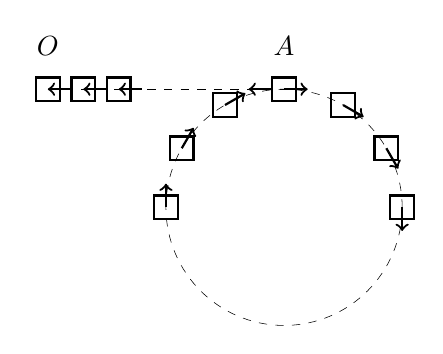
\begin{tikzpicture}[scale=1.5]
  % trace
  \draw[dashed, very thin] (-2cm, 1cm) -- (0, 1cm);
  \draw[dashed, very thin] (0,0) circle [radius=1cm];

  % leading nodes
  \foreach \x in {-2, -1.7, ..., -1.4} {
    \draw[thick] (\x cm, 1cm) +(-0.1, -0.1) rectangle ++(0.1, 0.1);
    \draw[thick, <-] (\x cm, 1cm) -- +(0.2, 0);
  }

  % cricular starting points
  \draw[thick, <-] (-0.3cm, 1cm) -- (-0.1cm, 1cm);

  \draw (-2cm, 1.2cm) node[above]{$O$};
  \draw (0, 1.2cm) node[above]{$A$};

  % circular nodes
  \foreach \deg/\rot in {90/0, 60/-30, 30/-60, 0/-90, 180/90, 150/60, 120/30} {
    \draw[thick] (\deg : 1cm) +(-0.1, -0.1) rectangle ++(0.1, 0.1);
    \draw[thick, ->] (\deg : 1cm) -- +(\rot : 0.2);
  }
\end{tikzpicture}
}

\subcaptionbox{Stage 2, the circle part is reversed}{
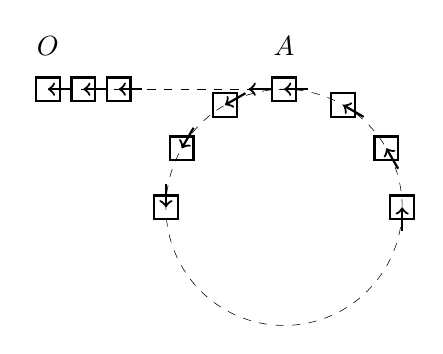
\begin{tikzpicture}[scale=1.5]
  % trace
  \draw[dashed, very thin] (-2cm, 1cm) -- (0, 1cm);
  \draw[dashed, very thin] (0,0) circle [radius=1cm];

  % leading nodes
  \foreach \x in {-2, -1.7, ..., -1.4} {
    \draw[thick] (\x cm, 1cm) +(-0.1, -0.1) rectangle ++(0.1, 0.1);
    \draw[thick, <-] (\x cm, 1cm) -- +(0.2, 0);
  }

  % cricular starting points
  \draw[thick, <-] (-0.3cm, 1cm) -- (-0.1cm, 1cm);

  \draw (-2cm, 1.2cm) node[above]{$O$};
  \draw (0, 1.2cm) node[above]{$A$};

  % circular nodes
  \foreach \deg/\rot in {90/0, 60/-30, 30/-60, 0/-90, 180/90, 150/60, 120/30} {
    \draw[thick] (\deg : 1cm) +(-0.1, -0.1) rectangle ++(0.1, 0.1);
    \draw[thick, <-] (\deg : 1cm) -- +(\rot : 0.2);
  }
\end{tikzpicture}
}

\subcaptionbox{Stage 3, The nodes between the original head and the circle is reversed back}{
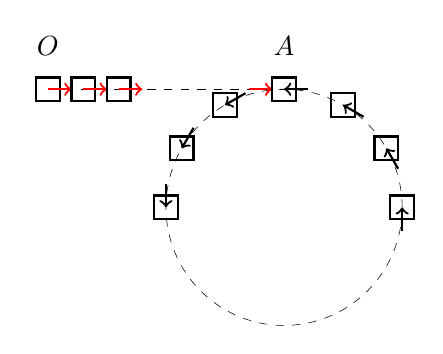
\begin{tikzpicture}[scale=1.5]
  % trace
  \draw[dashed, very thin] (-2cm, 1cm) -- (0, 1cm);
  \draw[dashed, very thin] (0,0) circle [radius=1cm];

  % leading nodes
  \foreach \x in {-2, -1.7, ..., -1.4} {
    \draw[thick] (\x cm, 1cm) +(-0.1, -0.1) rectangle ++(0.1, 0.1);
    \draw[red, thick, ->] (\x cm, 1cm) -- +(0.2, 0);
  }

  \draw (-2cm, 1.2cm) node[above]{$O$};
  \draw (0, 1.2cm) node[above]{$A$};

  % cricular starting points
  \draw[red, thick, ->] (-0.3cm, 1cm) -- (-0.1cm, 1cm);

  % circular nodes
  \foreach \deg/\rot in {90/0, 60/-30, 30/-60, 0/-90, 180/90, 150/60, 120/30} {
    \draw[thick] (\deg : 1cm) +(-0.1, -0.1) rectangle ++(0.1, 0.1);
    \draw[thick, <-] (\deg : 1cm) -- +(\rot : 0.2);
  }
\end{tikzpicture}
}
\caption{Reverse a circular list.}
\label{fig:reverse}
\end{figure}

After all the pointers being reversed in stage 1 and 2, the reversing doesn't
stop, but goes along with the line $AO$. Since all the nodes in section $AO$
have already been reversed, these pointers are restored. We can compare if
the new head is changed to tell if there is a cycle. After that, we need
perform another reversing to restore the linked-list back.

The following ANSI C code implements this solution.

\lstset{language=C}
\begin{lstlisting}
struct Node* reverse(struct Node* h) {
    struct Node *p = h, *h1 = NULL;
    while (h) {
        h = p->next;
        p->next = h1;
        h1 = p;
        p = h;
    }
    return h1;
}

int detect(struct Node* h) {
    struct Node* h1 = reverse(h);
    reverse(h1); /*resume the original list*/
    return h == h1;
}
\end{lstlisting}


\section{Cycle detection}
Circular list is a special case of general Cycle detection problem \cite{wiki-cycle-detection}.
For any function $f$ maps finite set $S$ to itself with any initial value $x_0$, the sequence of the
iteration:

\[
x_0, x_1 = f(x_0), x_2 = f(x_1), ...
\]

must repeat. between some $i \neq j$, $x_i = x_j$. The cycle detection problem is to find $i$ and $j$ for
given $f$ and $x_0$. The first method described here is invented by Robert W. Floyd in later 1960s, as known
as the `tortoise and the hare' algorithm.

For the circular list problem, the $f$ is defined as

\begin{equation}
f(x) = \left \{
  \begin{array}
  {r@{\quad:\quad}l}
  next(x) & x \neq NIL \\
  NIL & otherwise
  \end{array}
\right.
\end{equation}

The formalized Floyd's algorithm and Brent's algorithm are given as below. They accept the initial value
$x_0$, and the function $f$, return $k$ and $n$, where $k$ is the value the cycle starts and $n$ is the
period of the cycle.

\begin{algorithmic}[1]
\Function{Floyd-Cycle-Detection}{$x_0, f$}
  \State $p \gets q \gets x_0$ \Comment{$p$: the slow (tortoise), $q$: the fast (hare)}
  \Repeat
    \State $p \gets f(p)$
    \State $q \gets f(f(q))$
  \Until{$p = q$} \Comment{Loop until converge}
  \Statex
  \State $k \gets 0$
  \State $q \gets x_0$ \Comment{Reset the fast}
  \While{$p \neq q$} \Comment{Loop to the connection point}
    \State $p \gets f(p)$
    \State $q \gets f(q)$
    \State $k \gets k + 1$
  \EndWhile
  \Statex
  \State $n \gets 0$
  \Repeat \Comment{Traverse the circle}
    \State $q \gets f(q)$
    \State $n \gets n + 1$
  \Until{$q = p$}
  \State \Return $(k, n)$
\EndFunction
\end{algorithmic}

\begin{algorithmic}[1]
\Function{Brent-Cycle-Detection}{$x_0, f$}
  \State $n \gets 0, m \gets 1$
  \State $p \gets q \gets x_0$
  \Repeat{}
    \If{$m = n$}
      \State $p \gets q$ \Comment{Reset the start point}
      \State $n \gets 0$
      \State $m \gets 2m$
    \EndIf
    \State $q = f(q)$
    \State $n \gets n + 1$
  \Until{$p = q$} \Comment{Loop until converge}
  \Statex
  \State $ p \gets q \gets x_0$ \Comment{Reset}
  \Loop{ $n$ times} \Comment{Make distance $|qp| = n$}
    \State $q \gets f(q)$
  \EndLoop
  \Statex
  \State $k \gets 0$
  \While{$p \neq q$} \Comment{Loop to the connection point}
    \State $p \gets f(p)$
    \State $q \gets f(q)$
    \State $k \gets k + 1$
  \EndWhile
  \State \Return $(k, n)$
\EndFunction
\end{algorithmic}

\section{Functional approach}
\subsection{Floyd's algorithm}
The cycle detection solution can be defined in purely functional form. For Floyd's method, we
need define a function $converge(a, b)$. It applies function $f$ to $a$, and applies $f$ twice
to $b$. This function recursively finds the converge point where $a = b$.

\begin{equation}
converge(a, b) = \left \{
  \begin{array}
  {r@{\quad:\quad}l}
  a & a = b \\
  converge(f(a), f(f(b))) & otherwise
  \end{array}
\right.
\end{equation}

The converge point is given as $x_i = converge(x_1, x_2)$, where $x_1 = f(x_0)$ and $x_2 = f(x_1)$.
After that, we start iterating from $x_0$ and $x_i$ in parallel to find the connection point $x_k$.

\begin{equation}
connect(a, b, k) = \left \{
  \begin{array}
  {r@{\quad:\quad}l}
  (k, a) & a = b \\
  connect(f(a), f(b), k + 1) & otherwise
  \end{array}
\right.
\end{equation}

Because iterating $f$ on $x_0$ of $k$ times will arrive at the connection point $A$, and so as
from the converge point $x_i$. This function returns a pair of values $(k, x_k) = connect(x_0, x_i, 0)$, where the third parameter zero is the initial value for accumulating $k$.

The connection point $x_k$ is the place from where we can traverse the cycle to
count for $n$.

\begin{equation}
traverse(a) =  \left \{
  \begin{array}
  {r@{\quad:\quad}l}
  1 & a = x_k \\
  1 + traverse(f(a)) & otherwise
  \end{array}
\right.
\end{equation}

The final Floyd's algorithm can be realized as below.

\begin{equation}
floyd(x_0, f) = (k, n)
\end{equation}

Where
\[
\left \{
\begin{array}{l}
(k, x_k) = connect(x_0, converge(f(x_0), f(f(x_0))), 0) \\
n = traverse(x_k)
\end{array}
\right .
\]

The following Haskell example program implements this algorithm.

\lstset{language=Haskell}
\begin{lstlisting}
findCycle x0 f = (k, n) where
  (k, p) = connect x0 (converge (f x0) (f $ f x0)) 0
  n = traverse (f p)
  converge a b | a == b = a
               | otherwise = converge (f a) (f $ f b)
  connect a b cnt | a == b = (cnt, a)
                  | otherwise = connect (f a) (f b) (cnt + 1)
  traverse a | a == p = 1
             | otherwise = 1 + traverse (f a)
\end{lstlisting}

In the environments that support lazy evaluation, the solution can also be realized using infinite series.
Denote $X = \{x_0, x_1, x_2, ...\}$, and $X' = \{ x_1, x_2, ...\}$.
Taking the even number indexed elements yields $Y = \{x_0, x_2, x_4, ...\}$, and let $Y' = \{x_2, x_4, ...\}$
be the rest elements in $Y$. $Y$ contains all the possible values that applies $f$ twice from $x_0$.
If we pairing $X'$ and $Y'$, as $zip(X', Y') = \{(x_1, x_2), (x_2, x_4), ... (x_j, x_{2j}), ...\}$,
we can examine the pairs one by one till the converge point where the two values in the pair are equal.
Dropping all the examined pairs, we will have an infinite series of pairs from the converge point

\begin{equation}
\begin{array}{rl}
zip(C, D) & = \{(x_i, x_i), (x_{i+1}, x_{2(i+1)}), ...\} \\
  & = dropWhile(\lambda_{(x_j, x_k)} \cdot x_j \neq x_k, zip(X', Y'))
\end{array}
\end{equation}

Thus $C = \{x_i, x_{i+1}, ...\}$. At this stage, we can pairing $X$ and $C$, as
$zip(X, C) = \{(x_0, x_i), (x_1, x_{i+1}), ...\}$, to search the connection point
where the two values in the pair are equal. Then
we break the infinite series into two parts $Z_1, Z_2$, the first part contains elements before the
connection point $A$. The length of it is $k = |Z_1|$. And we can count the cycle from the second part.

\begin{equation}
(Z_1, Z_2) = span(\lambda_{(x_i, x_j)} \cdot x_i \neq x_j, zip(X, C))
\end{equation}

In order to find the cycle in $Z_2 = \{(x_k, x_k), (x_{k+1}, x_{k+1}), ...\}$, we examine from the second
pair one by one till meeting $(x_k, x_k)$ again.

\begin{equation}
n = 1 + |takeWhile(\lambda_{(x_i, x_j)} \cdot x_i = x_j = x_k, Z_2')|
\end{equation}

Where $Z_2'$ contains all the pairs from the second one in $Z_2$. The following Haskell example program
combines these ideas.

\lstset{language=Haskell}
\begin{lstlisting}
neq (x, y) = x /= y

findCycle' x0 f = (length sec, length cycle) where
  xs@(x:xs') = iterate f x0
  ys@(y:ys') = iterate (f.f) x0
  converge = fst $ unzip $ dropWhile neq (zip xs' ys')
  (sec, (z:zs)) = span neq (zip xs converge)
  cycle = z : takeWhile (z /=) zs
\end{lstlisting}

\subsection{Brent's algorithm}
In Brent's algorithm, the cycle period $n$ is calculated first. We define a function $converge(a, b, n, m)$.
Let $m$ be the power of 2 series $1, 2, 4, 8, ...$, and check if it converges within $m$ recursions.

\begin{equation}
converge(a, b, n, m) = \left \{
  \begin{array}
  {r@{\quad:\quad}l}
  converge(a, f(a), 1, 2m) & n = m \\
  n & a = b \\
  converge(a, f(a), n+1, m) & otherwise
  \end{array}
\right.
\end{equation}

If $n=m$, it can't converge in $m$ steps. We reset the start point to $a$, the period counter
$n$ to 1, and try again in next $2m$ steps; When $a = b$, it converges. $n$ records the circumference; Other
wise, we step ahead. The cycle length $n$ is given as $n = converge(x_0, f(x_0), 1, 1)$.

With $n$ calculated, we can get $k$ by finding the connection point $k = connect(x_0, f^n(x_0))$, where
$f^n(x_0)$ means applying function $f$ to $x_0$ with $n$ times.

\begin{equation}
connect(a, b) = \left \{
  \begin{array}
  {r@{\quad:\quad}l}
  0 & a = b \\
  1 + connect(f(a), f(b))
  \end{array}
\right.
\end{equation}

The following Haskell example program implements Brent's algorithm.

\lstset{language=Haskell}
\begin{lstlisting}
detectCycle x0 f = (k, n) where
  n = converge x0 (f x0) 1 1
  q = foldr ($) x0 (replicate n f)
  k = connect x0 q
  connect p q | p == q = 0
              | otherwise = 1 + connect (f p) (f q)
  converge p q n m | n == m = converge q (f q) 1 (2*m)
                   | p == q = n
                   | otherwise = converge p (f q) (n + 1) m
\end{lstlisting}

Brent's algorithm can be realized with infinite series as well in the programming environment that supports
lazy evaluation. We start $m$ from 1, then 2, 4, ... For each value, we search the converge point in
a section series of length $m$. For any given infinite values $Y = \{y_1, y_2, y_3, ...\}$, let
$Y' = \{y_2, y_3, ...\}$. We split $Y'$ at position $m$,
$(Y_1, Y_2) = splitAt(m, Y')$. Then we search $y_1$ in $Y_1$. If we fail to find it, we need
recursively search the converge point in a section of length $2m$ in $Y_2$. Otherwise the
position of $y_1$ in $Y_1$ is the length of the cycle.

\begin{equation}
converge(Y, m) = \left \{
  \begin{array}
  {r@{\quad:\quad}l}
  i & y_1 = y_i, y_i \in Y_1 \\
  converge(Y_2, 2m) & y_1 \notin Y_1
  \end{array}
\right.
\end{equation}

With $n$ calculated, we can get $k$ like below.

\begin{equation}
k = |takeWhile(\lambda_{(x_i, x_j)} \cdot x_i \neq x_j, zip(\{x_0, x_1, ... \}, \{x_{n}, x_{n+1}, ...\}))|
\end{equation}

The following Haskell example program implements this method by using infinite series and lazy evaluation.

\lstset{language=Haskell}
\begin{lstlisting}
detectCycle' x0 f = (k, n) where
  xs = iterate f x0
  n = converge xs 1
  k = length $ takeWhile neq (zip xs (drop n xs))
  converge (x:xs) m = let
      (ys, zs) = splitAt m xs in
      case elemIndex x ys of
        Nothing -> converge zs (2*m)
        (Just idx) -> idx + 1
\end{lstlisting}

The complete ANSI C and Haskell example programs with test are distributed with this article.

\begin{thebibliography}{99}

\bibitem{Stepanov09}
Alexander Stepanov, Paul McJones. ``Elements of Programming''. Section 2.3, Chapter 2. Addison-Wesley Professional; (2009)

\bibitem{TAOCP2}
Donald E. Knuth. ``The Art of Computer Programming, Volume 2: Seminumerical Algorithms (3rd Edition)''. Addison-Wesley Professional; (1997)

\bibitem{wiki-cycle-detection}
Cycle detection. Wikipedia. \url{https://en.wikipedia.org/wiki/Cycle_detection}

\end{thebibliography}

\end{document}
